\documentclass[10pt]{article}
\usepackage{graphicx}
\usepackage{amsfonts}
\usepackage{pifont}
\newcommand{\cmark}{\ding{51}}%
\newcommand{\xmark}{\ding{55}}%

\linespread{1}
\addtolength{\oddsidemargin}{-2.5cm}
%\addtolength{\evensidemargin}{-3cm}
\addtolength{\textwidth}{2.5cm}
\begin{document}



\begin{figure}
\caption{Median run times, in minutes, for the analysis of association study data from the six simulation scenarios. 
Eagle is compared against five other multiple-locus programs (top left plot) and two single-locus programs (top right plot). 
The x- and y-axes are on a log scale for improved aesthetics. Eagle has the lowest run-times of the multiple-locus 
programs, sometimes by orders of magnitude. Eagle can even produce results faster than single-locus programs. 
The actual median run times for the programs across the scenarios are given in the table. The entries in a bold font 
correspond to the lowest run-time for a scenario. 
 FaST-LMM$^{all}$ is where the single-locus results are based on all the available 
SNP data. FaST-LMM$^{few}$ is where the single-locus results as based on a subset of the available SNP data. }

\label{fig_time}
\begin{center}
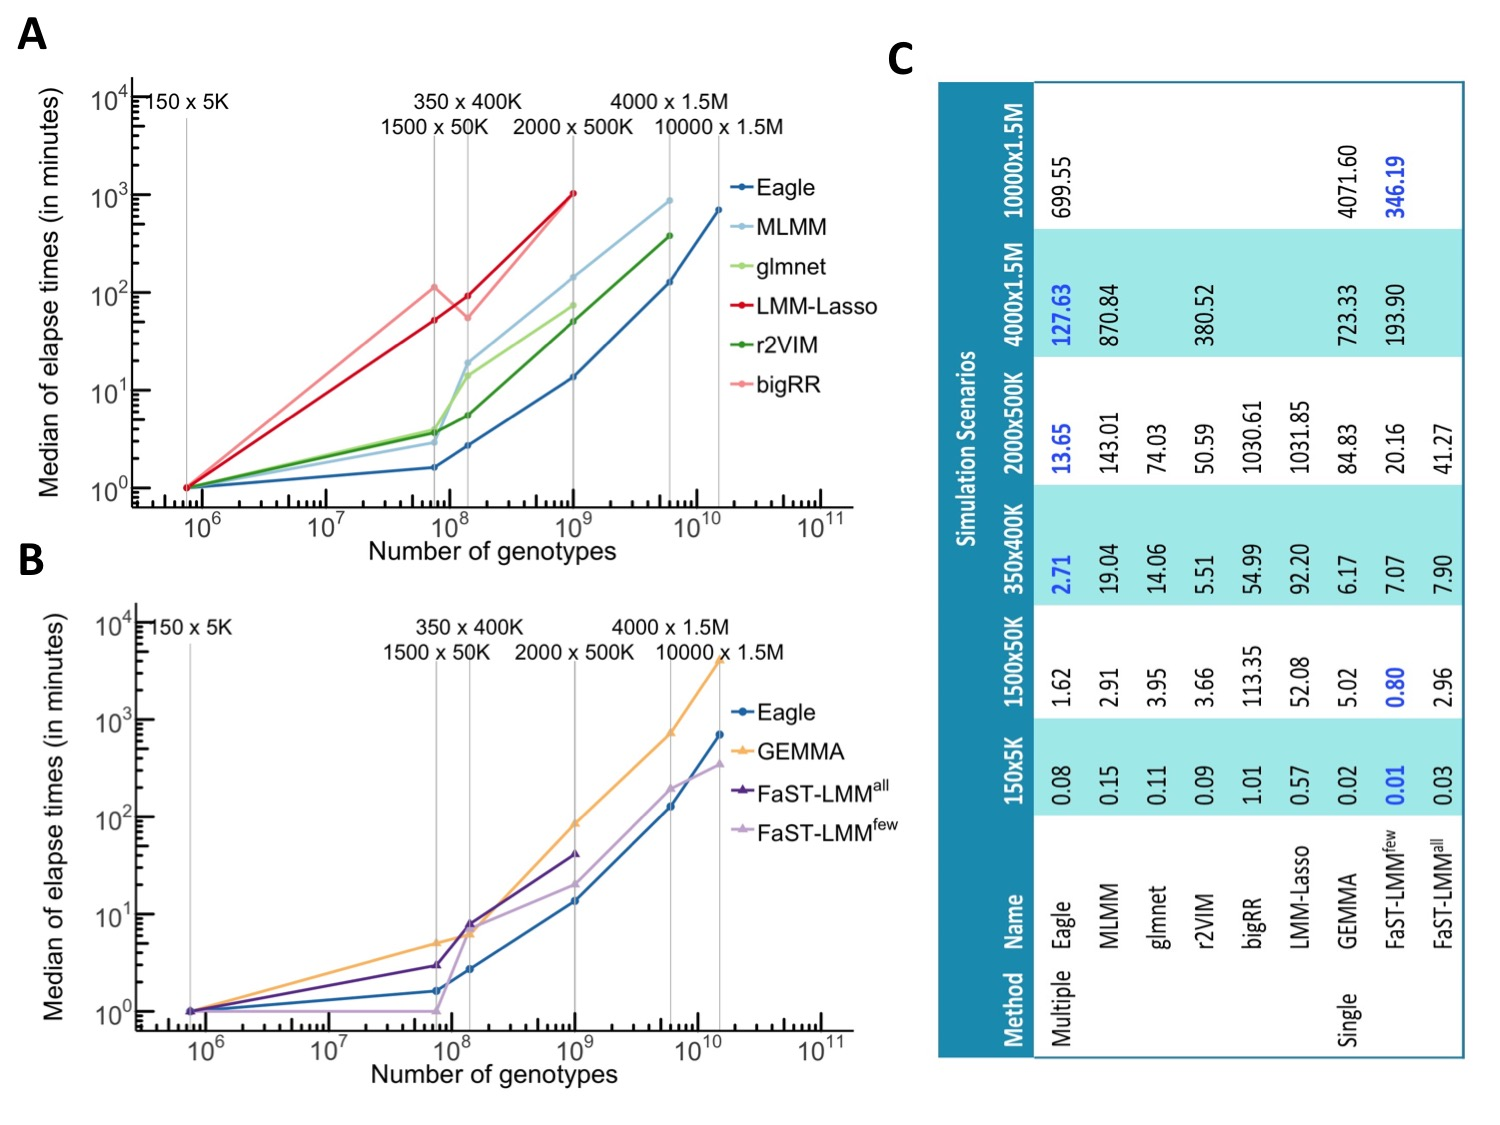
\includegraphics[width=12cm, height=12cm]{Figure2_time.jpg}
\end{center}

\end{figure}





\end{document}
